% Stroke threshold sweep on sheet08 (data: results/pencil-sheet08-overlap/protection-sweep.json).
% Same palette and fonts as the block diagrams. Build: tectonic bleed/diagrams/tradeoff.tex
\documentclass[border=8pt]{standalone}
\usepackage{amsmath}
\usepackage{pgfplots}
\pgfplotsset{compat=1.17}
\definecolor{blockedge}{HTML}{7FA7D9}
\definecolor{navy}{HTML}{1F3B73}
\definecolor{grey}{HTML}{8A94A3}

\begin{document}
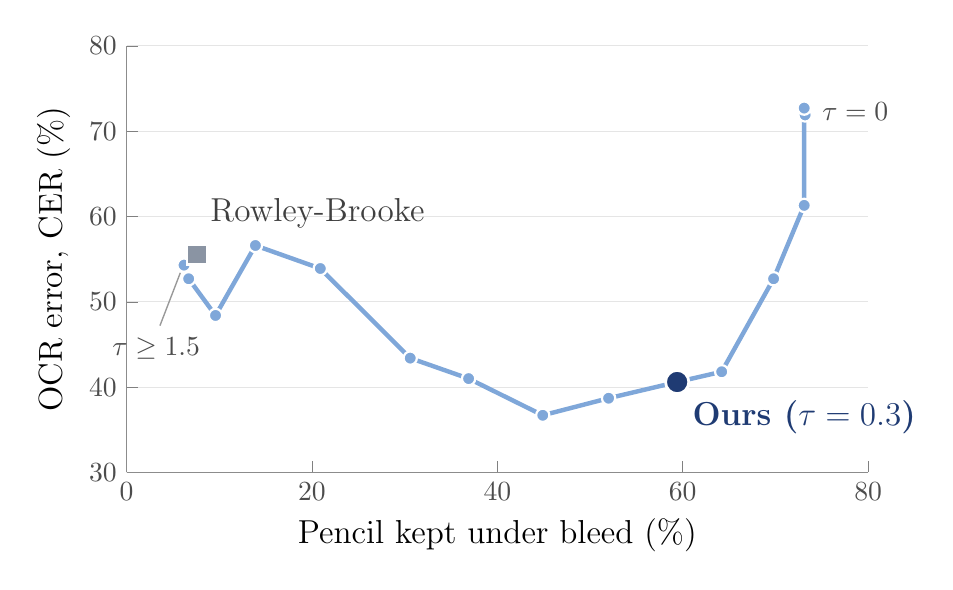
\begin{tikzpicture}
\begin{axis}[
    width=11cm, height=7cm,
    xmin=0, xmax=80, ymin=30, ymax=80,
    xtick={0,20,40,60,80}, ytick={30,40,50,60,70,80},
    xlabel={Pencil kept under bleed (\%)},
    ylabel={OCR error, CER (\%)},
    label style={font=\large}, tick label style={font=\normalsize, color=black!70},
    axis lines*=left, axis line style={color=black!45},
    ymajorgrids, grid style={color=black!10},
    clip=false,
]
  % tau sweep (anchored stroke mask), ordered by tau = 0 ... 1.5 (tau >= 1.5 protects nothing)
  \addplot[color=blockedge, line width=1.6pt, mark=*, mark size=2.4pt,
           mark options={fill=blockedge, draw=white, line width=0.8pt}]
    coordinates {(73.2,71.9) (73.1,72.7) (73.1,61.3) (69.8,52.7) (64.2,41.8) (59.4,40.6) (52.0,38.7) (44.9,36.7)
                 (36.9,41.0) (30.6,43.4) (20.9,53.9) (13.9,56.6) (9.6,48.4) (6.7,52.7) (6.2,54.3)};
  \node[anchor=west, color=black!70] at (axis cs:74.0,72.3) {$\tau=0$};
  \node[anchor=north, color=black!70] at (axis cs:3.2,47.0) {$\tau\geq1.5$};
  \draw[black!40, line width=0.5pt] (axis cs:3.6,47.2) -- (axis cs:5.8,53.4);

  % ours (default) and the paper
  \addplot[only marks, mark=*, mark size=4.2pt, color=navy, mark options={draw=white, line width=1pt}]
    coordinates {(59.4,40.6)};
  \node[anchor=north west, color=navy, font=\bfseries\large] at (axis cs:60.0,39.6) {Ours ($\tau=0.3$)};
  \addplot[only marks, mark=square*, mark size=3.6pt, color=grey, mark options={draw=white, line width=1pt}]
    coordinates {(7.6,55.5)};
  \node[anchor=south west, color=black!75, font=\large] at (axis cs:8.0,57.5) {Rowley-Brooke};
\end{axis}
\end{tikzpicture}
\end{document}
